%% OrchestraBench --- DAI 2026 submission (full-content draft).
%% Template: ACM acmart (DAI 2026 proceedings go through ACM ICPS).
%% `nonacm` keeps this a clean draft (no ACM conference/copyright block);
%% remove `nonacm` and add the DAI \acmConference{} metadata for camera-ready.
%% Local compile: tectonic -p paper/main.tex (see README.md).
\documentclass[sigconf,nonacm,anonymous]{acmart}  % anonymous = double-blind submission; remove `anonymous` for camera-ready (restores authors + acks)

\usepackage{booktabs}
\usepackage{graphicx}
\graphicspath{{../figures/}{./figures/}{./}}

\settopmatter{printacmref=false}

\begin{document}

\title{OrchestraBench: Evaluating Multi-Agent Orchestration Failure
Modes, Recovery, and Decomposition Quality}

\author{Yidian Chen}
\affiliation{%
  \institution{Anote}
  \country{}
}
\author{Yingzi Gu}
\affiliation{%
  \institution{Anote}
  \country{}
}

\begin{abstract}
Multi-agent orchestration frameworks (AutoGen, LangGraph, CrewAI, Anthropic
Agents SDK) are moving from demos to production, yet they can only be compared
on \emph{task accuracy} --- not on \emph{reliability}. Existing agent benchmarks
measure whether a pipeline succeeds, but cannot diagnose \emph{why} it failed,
\emph{where} a cascade began, or \emph{which} routing decision caused the
breakdown. We present \textbf{OrchestraBench}, a benchmark that evaluates
how multi-agent systems \textbf{fail, recover, and decompose} as first-class,
comparable metrics. OrchestraBench contributes (i) a controlled,
seed-reproducible \textbf{failure-injection harness} over templated enterprise
workflows, (ii) \textbf{cascade-radius} and per-failure-mode recovery as primary
metrics, and (iii) a \textbf{routing-policy comparison} with bootstrap
confidence intervals and paired tests where applicable. Our first experiment
isolates the routing-mechanism question: on a
26-case gold-labelled diagnostic, a keyword/flag heuristic --- representative of
production rule-based routers --- scores \textbf{0\% on adversarial cases}
(misleading or missing surface flags), while a model-driven router that reasons
over intent scores \textbf{100\%}, matching the oracle on this diagnostic.
This indicates that the heuristic's blind spot is a property of the routing
\emph{mechanism}, not the diagnostic's inherent difficulty. Two further
experiments, run
with a real Claude agent over a \textbf{verifiable arithmetic dependency chain}
as a controlled mechanism probe, quantify a reliability axis existing benchmarks
leave undermeasured: across five MAST failure modes, the four latent/semantic
modes fail completely (final-task success \textbf{0.0}) while a tool fault is
fully recovered (\textbf{1.0}), and \textbf{retry does not repair the latent
modes} --- it extends a corrupted trace rather than containing it; and cascade
radius \textbf{scales monotonically with pipeline depth} (mean 1.0 / 2.9 / 5.0
at depths 3 / 5 / 7) --- the stages-traversed signature MAS-FIRE leaves
unquantified. A policy-conditioned extension further suggests that containment
can improve under a stronger self-correction semantics: with trusted upstream
state, an LLM router cuts latent cascade radius $\sim$5.5$\times$ over rule-based
baselines at depth 7 --- but an ablation shows this gain is largely the
trusted-state signal, not autonomous detection. We frame these as controlled-chain mechanism probes, not
domain-workload claims (\S\ref{sec:limitations}).
\end{abstract}

\keywords{LLM orchestration, multi-agent systems, benchmarking, failure
recovery, cascade propagation}

\maketitle

\section{Introduction}
Multi-agent systems increasingly orchestrate several specialized agents ---
routers, retrievers, tool-callers, planners --- behind a single task. When such
a pipeline produces a wrong or low-quality answer in production, the failure is
often \emph{silent}: a misrouted task still yields a plausible-looking response.
Current benchmarks (AgentBench~\cite{agentbench}, OdysseyBench~\cite{odysseybench},
SWE-Bench~\cite{swebench}) report final task success and so cannot tell teams
\textbf{which} orchestration decision failed, \textbf{how far} an error
propagated, or \textbf{whether} intelligent routing was worth its added
complexity. This
blocks the most basic production decision: choosing and hardening an
orchestration framework on \emph{reliability} rather than ergonomics.

\paragraph{Contributions.}
\begin{enumerate}
  \item \textbf{OrchestraBench}, a benchmark that treats orchestration
  \emph{failure handling} as the unit of evaluation: controlled failure
  injection, per-failure-mode recovery, and cascade propagation.
  \item A \textbf{seed-reproducible} workflow + failure-injection harness
  (scenarios regenerable from seeds; aggregates recomputable from committed
  artifacts) with templated enterprise workflow families.
  \item A \textbf{routing-policy comparison} (Fixed / Heuristic / LLM / Oracle)
  with bootstrap confidence intervals and paired significance testing where
  applicable, isolating \emph{when} intelligent routing beats a zero-decision
  baseline.
\end{enumerate}

\paragraph{Research questions.}
\begin{itemize}
  \item \textbf{RQ1 (routing value)}: When does intelligent routing (heuristic or
  LLM) actually beat a zero-decision baseline?
  \item \textbf{RQ2 (mechanism)}: Is routing reliability a property of task
  \emph{difficulty}, or of the routing \emph{mechanism} (keyword/flag matching
  vs.\ reasoning over intent)? \emph{(Answered by Exp 1.)}
  \item \textbf{RQ3 (attribution)}: Can a pipeline failure be attributed to a
  specific failure mode \emph{and} stage, reproducibly across runs?
  \item \textbf{RQ4 (cascade)}: How far does a single seeded error propagate
  downstream, and which routing/recovery strategies contain it?
\end{itemize}

\section{Related Work}
\label{sec:related}
OrchestraBench sits among recent work that \emph{observes}, \emph{attributes}, or
\emph{proposes} fixes for multi-agent failure; we differ by making controlled
injection, cascade radius, and routing-policy mechanism the unit of analysis
(Table~\ref{tab:related}).

\begin{table*}[t]
\centering
\caption{OrchestraBench versus closely related work.}
\label{tab:related}
\small
\begin{tabular}{@{}p{3.4cm}p{6.0cm}p{6.0cm}@{}}
\toprule
\textbf{Prior work} & \textbf{What it does} & \textbf{How OrchestraBench differs} \\
\midrule
MAST~\cite{mast} (14 failure modes, 1{,}600+ traces, $\kappa{=}0.88$) &
Empirically-grounded \emph{taxonomy} of observed MAS failures &
We \emph{inject} that taxonomy under seed-controlled conditions and measure
recovery + cascade \emph{per mode} --- MAST observes, we intervene \\
MAS-FIRE~\cite{masfire} &
Fault injection + reliability evaluation; intra-/inter-agent fault taxonomy &
\textbf{Closest prior work} (\S\ref{sec:novelty}). We differ on emphasis: cascade
\emph{radius across pipeline depths} + \emph{routing-policy comparison} as the
unit of analysis, not reliability scoring alone \\
TraceElephant~\cite{traceelephant} (220 annotated traces) &
Benchmark for post-hoc failure attribution in MAS &
Attribution is observational; we add controlled seeding + cascade radius as
\emph{primary} metrics \\
Agents Failure Attribution~\cite{attribution} (Who\&When; 127 MAS) &
Post-hoc attribution to the responsible agent/step &
Same: attribution is a means here, not the product \\
Orchestration-pattern benchmark~\cite{orchpattern} (10k SEC filings) &
Compares sequential / parallel / hierarchical / reflexive architectures on a
cost-accuracy Pareto &
Architecture comparison on accuracy/cost; we evaluate \emph{failure handling} and
routing \emph{mechanism} --- complementary \\
AdaptOrch~\cite{adaptorch} &
Task-adaptive orchestration \emph{framework} (+12--23\%) &
A method; OrchestraBench is the benchmark that would evaluate it \\
From Spark to Fire~\cite{sparkfire} &
Errors cascade exponentially in pipelines &
We operationalize this into a measurable cascade-radius benchmark \\
\bottomrule
\end{tabular}
\end{table*}

\paragraph{Motivating data point.} \emph{Beyond the
Strongest}~\cite{beyondstrongest} reports that on GPQA-Diamond at least one agent
was correct in \textbf{95.5\%} of cases, yet orchestration reached only
\textbf{87.4\%} --- i.e.\ orchestration \emph{discards} $\sim$8 points of
individually-recoverable correctness. OrchestraBench is built to attribute
exactly this loss.

\paragraph{The gap.} Existing work either \emph{observes} failures
(MAST~\cite{mast}), \emph{attributes} them post-hoc
(TraceElephant~\cite{traceelephant}, \cite{attribution}), or \emph{proposes}
better orchestration (AdaptOrch~\cite{adaptorch}). The one work that also
\emph{injects} (MAS-FIRE~\cite{masfire}) scores reliability but does not make
cascade radius or routing-policy mechanism its unit of analysis. OrchestraBench's
contribution is a \textbf{controlled, reproducible injection harness that
measures recovery and cascade containment as first-class metrics, compared across
routing policies.}

\subsection{Positioning Relative to Closest Prior Work}
\label{sec:novelty}
An honest audit (the space moved fast in early 2026) surfaces one direct overlap
and our response:
\begin{itemize}
  \item \textbf{MAS-FIRE~\cite{masfire} already performs controlled fault
  injection + reliability evaluation}, overlapping our Exp 2/3 substantially. Our
  differentiation is \emph{not} ``we inject failures'' (they do too); it is (a)
  \textbf{cascade radius across pipeline depths} as a first-class comparable
  metric, (b) failure handling measured \textbf{per routing policy}, and (c) the
  \textbf{routing-mechanism result} of Exp 1, which MAS-FIRE does not address. In
  our reading, MAS-FIRE does not quantify cascade depth as a stages-traversed
  metric and does not vary routing policy; its axes are topology (MetaGPT /
  Table-Critic / CAMEL), fault-type (15), and model. OrchestraBench therefore
  complements MAS-FIRE by making cascade depth and routing policy first-class
  evaluation axes.
  \item \textbf{Attribution benchmarks~\cite{traceelephant,attribution} are
  observational/post-hoc} --- a different instrument from seeded, reproducible
  injection + recovery.
  \item \textbf{Internal overlap: IntentBench~\cite{intentbench}} evaluates
  whether the agent's \emph{understanding of intent} is correct (intent-spec vs.\
  syntactic tool-call correctness); OrchestraBench evaluates which
  \emph{orchestration action} to take given a correct understanding and how those
  decisions cascade. We measure the \textbf{decision policy and its failure
  propagation}, not intent correctness --- complementary ends of the pipeline,
  no measurement overlap.
\end{itemize}

\section{The OrchestraBench Benchmark}
\textbf{Workflow suites.} Synthetically generated from templated task graphs
(stages, inter-task dependencies, per-task \texttt{complexity\_score}), screened
by two annotators for realism. Three enterprise families: finance approval
(4 stages), HR onboarding (5 stages), DevOps deployment (5 stages).

\textbf{Routing decision space.} Each task is routed to one of four actions:
\texttt{DIRECT\_TOOL}, \texttt{CODE\_EXECUTION}, \texttt{DECOMPOSE},
\texttt{REASON\_ONLY}.

\textbf{Gold labels.} Routing and decomposition labels are produced
independently by two annotators with adjudication on disagreement.

\textbf{Failure injection.} Failure scenarios are seeded \textbf{deterministically}
on top of the suites via the \texttt{FailureInjector}, so each scenario is
reproducible from a seed.

\textbf{Metrics.} Primary reported metrics are routing accuracy,
per-failure-mode recovery rate, \textbf{cascade radius}, time-to-detection,
recovery completeness, and decomposition delegation fidelity. The harness also
records routing macro-F1, per-class routing metrics, success rate, latency, cost,
and orchestration efficiency for larger suite-level comparisons.

\section{Experimental Setup}
\label{sec:setup}
\begin{table}[t]
\centering
\caption{Routing policies under comparison.}
\label{tab:policies}
\small
\begin{tabular}{@{}llp{3.4cm}@{}}
\toprule
\textbf{Policy} & \textbf{Type} & \textbf{What it tests} \\
\midrule
Fixed & Baseline & Zero-intelligence lower bound (always one route) \\
Heuristic & Baseline & Rule/keyword routing on complexity + flags \\
LLM-as-Router & Test & Model decides routing per task by reasoning over
description + metadata \\
Retry(heuristic) & Test & Adds automatic retry --- does retry alone contain
cascades? \\
Oracle & Ceiling & Routes to the gold label (upper bound) \\
\bottomrule
\end{tabular}
\end{table}
Reported confidence intervals use 95\% bootstrap CIs; paired bootstrap
significance tests ($\alpha = 0.05$) are used where paired comparisons are
defined.

\section{Results}
\label{sec:results}
\subsection{Experiment 1 --- Routing Policy Comparison (measured)}
We isolate the routing-mechanism question on a focused diagnostic of
\textbf{26 expert-labelled gold cases} covering all four routing decisions: 16
\emph{aligned} (surface flags match intent) and 10 \emph{adversarial} (flags
missing or misleading, but the description's intent is unambiguous). The
model-driven router is Claude Sonnet 4.6 via forced structured (tool-use) output;
results are stable across 3 independent passes (78/78), and the prompt never sees
the gold label.

\begin{table}[t]
\centering
\caption{Experiment 1: routing accuracy by case type.}
\label{tab:exp1}
\small
\begin{tabular}{@{}lccc@{}}
\toprule
\textbf{Policy} & \textbf{Overall} & \textbf{Aligned} & \textbf{Adversarial} \\
\midrule
Fixed & 23\% & 25\% & 20\% \\
Heuristic (keyword/flags) & 62\% & \textbf{100\%} & \textbf{0\%} \\
LLM-as-Router (Sonnet 4.6) & \textbf{100\%} & 100\% & \textbf{100\%} \\
Oracle (ceiling) & 100\% & 100\% & 100\% \\
\bottomrule
\end{tabular}
\end{table}

\textbf{Finding.} The heuristic is perfect on aligned cases but collapses to
\textbf{0\%} on adversarial ones; the model-driven router recovers \textbf{all} of
them (0\% $\to$ 100\%), matching the oracle on this diagnostic. Because the same
tasks are solved by an intent-reasoning router, the heuristic's adversarial
failure is best explained by the routing \textbf{mechanism} (keyword/flag
matching vs.\ reasoning over intent), not by inherent task difficulty. Larger
workflow-suite evaluation is the intended setting for a graded comparison once
the diagnostic no longer saturates.

\subsection{Experiment 2 --- Failure Injection and Recovery (real Claude
measured run; core)}
\textbf{Design.} Five MAST failure modes --- \emph{ambiguous delegation},
\emph{tool-invocation error}, \emph{context pollution}, \emph{conflicting
sub-agent outputs}, \emph{premature action} --- injected at the \textbf{prompt
level} into a verifiable arithmetic dependency chain executed by a \textbf{real
Claude agent} (Sonnet 4.6), under fixed, heuristic, and retry policies. Real
recovery / cascade are measured by exact-match against ground truth; the
measured-run module is included in the repository.

\begin{table}[t]
\centering
\caption{Experiment 2: per-mode final-task success and cascade radius, arithmetic
chain vs.\ loan-approval domain (real Claude, $N{=}30$ each; 95\% bootstrap CI).}
\label{tab:exp2}
\small
\begin{tabular}{@{}lcccc@{}}
\toprule
& \multicolumn{2}{c}{\textbf{Arithmetic}} & \multicolumn{2}{c}{\textbf{Domain}} \\
\cmidrule(lr){2-3}\cmidrule(lr){4-5}
\textbf{Failure mode} & \textbf{Success} & \textbf{Cascade} & \textbf{Success} &
\textbf{Cascade} \\
\midrule
tool\_invocation\_error & 1.00 & 0.00 & 0.67 & 0.67 \\
ambiguous\_delegation & 0.00 & 2.00 & 0.50 & 1.00 \\
context\_pollution & 0.00 & 2.00 & 0.00 & 2.00 \\
conflicting\_outputs & 0.00 & 2.00 & 0.00 & 2.00 \\
premature\_action & 0.00 & 2.00 & 0.00 & 2.00 \\
\bottomrule
\end{tabular}
\end{table}

\textbf{Real measured findings (Sonnet 4.6, $N{=}30$).}
The tool-invocation mode is \textbf{fully recovered} (recovery 1.0, cascade
radius 0) --- the agent computes by hand when the tool fails. The four
\textbf{latent/semantic modes} all \textbf{fail} (final-task success
\textbf{0.0}) and \textbf{cascade to every downstream stage} (cascade radius 2 of
2). Critically, the retry policy \textbf{does not recover them}: retrying
while the failure is still present reproduces the error and only
\textbf{lengthens time-to-detection}. This real-agent result supports the
mechanism: retry repairs retryable tool faults but not failures needing
attribution, state repair, or semantic validation (RQ3/RQ4). Bootstrap CIs are
degenerate here (latent modes 0.0 [0.0, 0.0]; tool fault 1.0 [1.0, 1.0], $n{=}6$
each), reflecting the controlled construct and small per-mode sample, not
statistical strength
(\S\ref{sec:limitations}).

\textbf{Domain-grounded validation (loan-approval workflow, $N{=}30$).} To test
whether these signatures are an artifact of the abstract arithmetic chain, we
re-ran the \emph{identical} failure injection on a domain-grounded variant: the
same verifiable computation reframed as a multi-role loan-approval pipeline
(Intake Officer $\to$ Risk Analyst $\to$ Compliance Officer $\to$ Approval
Manager), each stage prompted in business terms. \textbf{The core ordering
mostly holds}: context pollution, conflicting outputs, and premature action
still fail completely, while tool faults remain the most recoverable
(Figure~\ref{fig:exp2}). Crucially, the \textbf{absolute rates shift with
framing}: ambiguous delegation rises to \textbf{0.50} (the business-role
context lets the agent infer the intended operation about half the time) and
tool-invocation recovery falls to \textbf{0.67}. This
framing-sensitivity is evidence of model behavior under context, not a purely
structural tautology, and directly addresses the construct-validity concern
(\S\ref{sec:limitations}).

\begin{figure}[t]
\centering
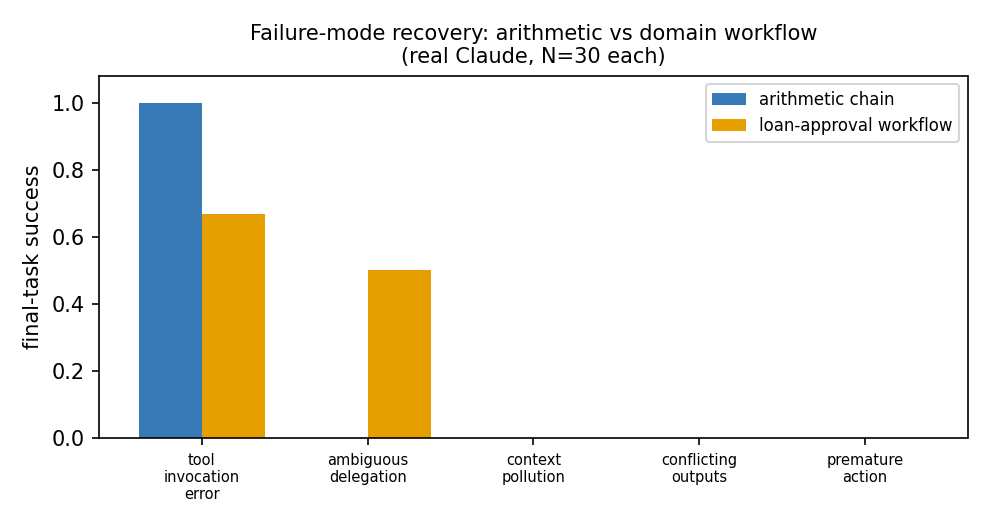
\includegraphics[width=\columnwidth]{exp2_arith_vs_domain.png}
\caption{Experiment 2 --- failure-mode final-task success, arithmetic chain vs.\
loan-approval workflow; the failure-mode \emph{ordering} is robust across framings
while absolute rates shift (real Claude, $N{=}30$ each).}
\label{fig:exp2}
\end{figure}

\subsection{Experiment 3 --- Cascade Propagation Depth (real Claude measured run,
$N{=}90$; core)}
\textbf{Design.} Inject a single seeded error at stage 1 of variable-depth
(3-, 5-, 7-stage) pipelines and measure how far it propagates. \textbf{Cascade
radius} (downstream stages corrupted) is a central differentiator vs.\ MAS-FIRE,
which has no stages-traversed metric.

\begin{table}[t]
\centering
\caption{Experiment 3: mean cascade radius by pipeline depth (real Claude,
$N{=}90$; latent modes pooled, $n{=}24$/depth; 95\% bootstrap CI). Linear in
depth: cascade $\approx$ depth $-$ 2.}
\label{tab:exp3}
\small
\begin{tabular}{@{}lcc@{}}
\toprule
\textbf{Depth} & \textbf{Latent cascade radius} & \textbf{Tool cascade radius} \\
\midrule
3 & 1.00 [1.00, 1.00] & 0.00 \\
5 & 2.88 [2.63, 3.00] & 0.00 \\
7 & 5.00 [5.00, 5.00] & 0.00 \\
\bottomrule
\end{tabular}
\end{table}

\textbf{Real measured findings (Sonnet 4.6, $N{=}90$).} Across the four
latent/semantic failure modes, \textbf{mean cascade radius scales monotonically
with depth: 1.0 $\to$ 2.9 $\to$ 5.0 at depths 3 / 5 / 7}
(Table~\ref{tab:exp3}, Figure~\ref{fig:exp3}) --- the failure propagates to
essentially every downstream stage (depth $-$ 2). Tool-invocation errors stay at
cascade radius 0 at every depth (the agent recomputes by hand). The lone
deviation is ambiguous delegation at depth 5 (mean 2.5 vs.\ 3.0 for the
other latent modes), where the real agent occasionally guesses the intended
operation correctly --- a realistic-noise signature absent from a deterministic
model. \textbf{This is the paper's main cascade-depth result and a primary
differentiator vs.\ MAS-FIRE.}

\begin{figure}[t]
\centering
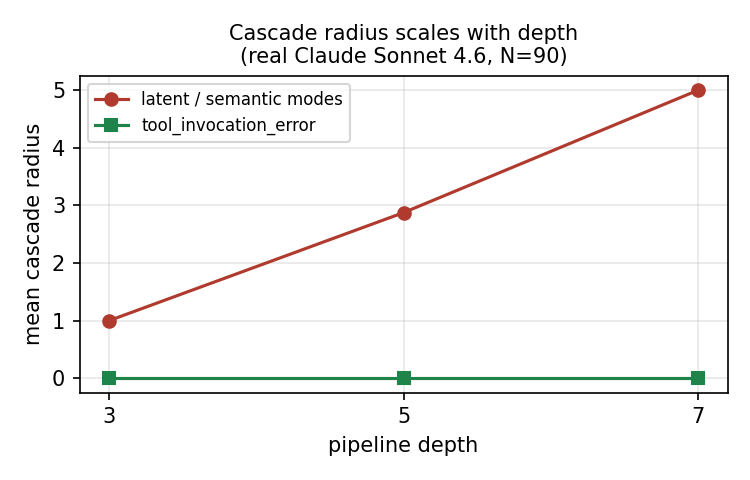
\includegraphics[width=\columnwidth]{exp3_cascade_by_depth.png}
\caption{Experiment 3 --- mean cascade radius vs.\ pipeline depth; latent/semantic
modes scale 1.0 $\to$ 2.9 $\to$ 5.0 across depths 3/5/7 while tool faults stay at
0 (real Claude, $N{=}90$).}
\label{fig:exp3}
\end{figure}

\subsection{Experiment 4 --- Decomposition Quality (real Claude measured run,
$N{=}20$; secondary)}
For composite tasks $(a \mathbin{op} b) \mathbin{op} (c \mathbin{op} d)$ with a
canonical 3-step gold decomposition, we score the produced decomposition against
gold --- \textbf{delegation fidelity} (gold sub-results recovered),
\textbf{granularity error}, \textbf{wasted sub-tasks} --- comparing a
\texttt{monolithic} (single-step) vs.\ a \texttt{decompose} (planner) policy.

\begin{table}[t]
\centering
\caption{Experiment 4: decomposition quality, decompose vs.\ monolithic (real
Claude, $N{=}20$; 95\% bootstrap CI). Paired bootstrap over the 10 shared tasks.}
\label{tab:exp4}
\small
\begin{tabular}{@{}lccc@{}}
\toprule
\textbf{Policy} & \textbf{Deleg.\ fidelity} & \textbf{Granularity err.} &
\textbf{Final correct} \\
\midrule
decompose & 1.00 [1.00, 1.00] & 0.00 [0.00, 0.00] & 1.00 \\
monolithic & 0.37 [0.33, 0.43] & 2.00 [2.00, 2.00] & 1.00 \\
\midrule
paired $\Delta$ & \multicolumn{3}{l}{fidelity $+0.63$ [0.57, 0.67], $p<0.0001$;
granularity $-2.0$, $p<0.0001$} \\
\bottomrule
\end{tabular}
\end{table}

\textbf{Real measured findings (Sonnet 4.6, $N{=}20$).} The \texttt{decompose}
policy produces a faithful three-step decomposition (delegation fidelity
\textbf{1.00}, granularity error \textbf{0}), while \texttt{monolithic} reaches
the correct final answer but exposes no delegable sub-structure (fidelity
\textbf{0.37 [0.33, 0.43]}, granularity error \textbf{2}). This fidelity gap is
large and statistically significant under a paired bootstrap over the 10 shared
tasks: \textbf{$+0.63$, 95\% CI [0.57, 0.67], $p<0.0001$}
(Table~\ref{tab:exp4}). Notably, \texttt{final\_correct} is \textbf{1.0 for both}
--- the arithmetic is easy enough that both get the answer; the discriminator is
the \textbf{decomposition structure}, not final correctness. For multi-agent
orchestration this is exactly the point: a monolithic agent can be \emph{right}
yet produce nothing a planner can delegate, audit, or recover from.

\subsection{Policy-conditioned containment probe (real Claude, $N{=}75 + N{=}225$)}
Experiments 2--3 pool over baseline policies; we add \textbf{LLM-as-router} and
\textbf{Oracle} policies to ask whether the routing policy itself can govern
containment. \textbf{The LLM-policy semantics are an explicit modelling
assumption}: at the injected stage the router is given the trusted upstream value
and licensed to detect and correct the anomaly. We therefore treat the LLM row as
a strong self-correction probe rather than a clean estimate of deployable routing
without trusted state.

\begin{table}[t]
\centering
\caption{Policy-conditioned containment on latent failures (real Claude, $N{=}75$; 95\% bootstrap CI).}
\label{tab:policy}
\small
\begin{tabular}{@{}lcc@{}}
\toprule
\textbf{Policy} & \textbf{Latent recovery} & \textbf{Cascade radius} \\
\midrule
fixed / heuristic / retry & 0.08 [0.00, 0.25] & 1.83 [1.50, 2.00] \\
\textbf{LLM-as-router} & \textbf{0.83 [0.58, 1.00]} & \textbf{0.33 [0.00, 0.83]} \\
Oracle (ceiling) & 1.00 [1.00, 1.00] & 0.00 [0.00, 0.00] \\
\bottomrule
\end{tabular}
\end{table}

\textbf{Policy probe by depth ($N{=}225$).} Under this stronger trusted-state
semantics, the policy effect \emph{amplifies with pipeline depth}: baseline
cascade radius grows with depth (0.9 / 2.7 / 4.6 at depths 3 / 5 / 7), while the
LLM router stays nearly flat (0.25 / 0.75 / 0.83) and Oracle fully contains (0 /
0 / 0). At depth 7 the LLM router cuts cascade radius
\textbf{$\sim$5.5$\times$} versus the baselines. This suggests that containment
benefits can become larger in deeper pipelines, while the deployable-routing
version remains future work (Figure~\ref{fig:policy}). The policy CSVs are
committed under \texttt{data/measured/}.

\textbf{Ablation: the model, or the hint?} The rows above hand the router the
trusted upstream value --- a possible information leak. Re-running Exp 2 with an
\texttt{llm\_noupstream} policy (same self-correction, \emph{no} trusted-upstream
hint) collapses latent recovery from \textbf{0.75 [0.50, 1.00]} to
\textbf{0.17 [0.00, 0.42]}, barely above the baseline 0.08 (paired drop
\textbf{0.58 [0.17, 0.92], $p<0.01$}). The LLM policy's containment is thus
\emph{mostly the trusted-upstream signal, not autonomous detection}: we read the
LLM column as a trusted-state probe, not evidence that an LLM router autonomously
contains latent cascades (\texttt{exp2\_ablation\_real.csv}).

\begin{figure}[t]
\centering
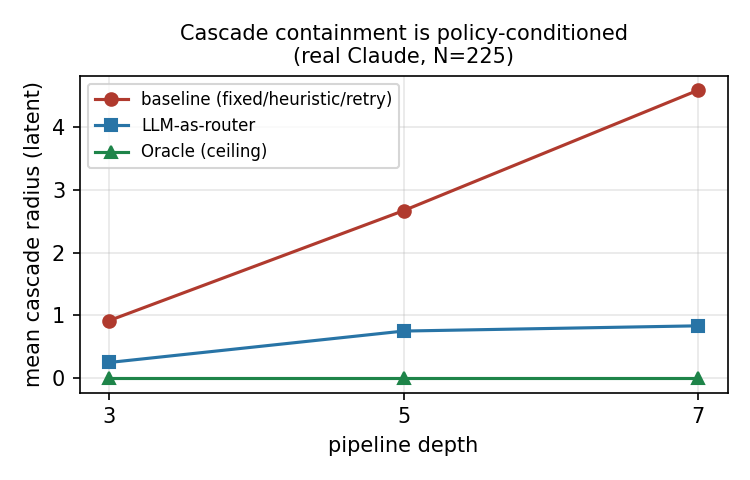
\includegraphics[width=\columnwidth]{exp3_policy_cascade.png}
\caption{Experiment 3 --- mean latent cascade radius vs.\ pipeline depth per
routing policy; baseline grows with depth while the trusted-state LLM probe stays
nearly flat and Oracle fully contains (real Claude, $N{=}225$).}
\label{fig:policy}
\end{figure}

\section{Discussion}
Experiment 1 establishes the paper's first reproducible claim: routing reliability
depends on \emph{mechanism}. Experiments 2 and 3 deliver the main reliability
result on a controlled verifiable chain: the \textbf{failure-mode gap} is
measured (four latent modes at 0.0 final-task success vs.\ a fully-recovered tool
fault), and \textbf{cascade radius scales with pipeline depth} (1.0 $\to$ 2.9
$\to$ 5.0 at depths 3 / 5 / 7) --- a stages-traversed signature not emphasized
by prior reliability benchmarks. Critically, \textbf{retry does not eliminate latent
cascades}: it reproduces the failure and lengthens time-to-detection, so
\emph{detection/attribution} --- not blind retry --- is the necessary containment
mechanism. The policy-conditioned extension shows the potential value of trusted
state repair, but its deployable interpretation is deliberately limited
(\S\ref{sec:limitations}). We are deliberate that these are mechanism probes on a
controlled chain; domain-workflow validation is the next step.

\section{Limitations}
\label{sec:limitations}
\begin{itemize}
  \item The Exp 1 diagnostic is small (26 cases) and \emph{saturates} for a
  capable model --- it is a mechanism probe, not a difficulty benchmark; the
  larger workflow-suite results are needed for a graded comparison.
  \item Workflows are synthetically generated; real-world pipeline validation is
  future work.
  \item Single model family reported for the LLM router; a cross-model sweep is
  future work.
  \item \textbf{Construct validity of Exp 2/3.} The failure-recovery and cascade
  experiments run on a \emph{verifiable arithmetic dependency chain}, chosen for
  clean ground truth, not a domain workflow. In this construct cascade radius is
  \textbf{partly by design} --- a downstream stage consumes the upstream value,
  so a latent corruption propagates to $\sim$(depth $-$ 2) stages --- so we
  present Exp 2/3 as \textbf{controlled mechanism probes}. The evidence that this
  measures model behavior rather than a tautology is the
  non-determinism we observe (ambiguous delegation at depth 5 yields
  mean cascade 2.88, below the structural maximum) and the domain-grounded re-run
  (Figure~\ref{fig:exp2}): the failure-mode \emph{ordering} mostly persists
  across framings while absolute rates shift with context. Full finance /
  HR / DevOps suite validation remains future work.
  \item \textbf{Single LLM, not a literal multi-agent system.} Exp 2/3 execute one
  Claude agent over a staged chain with prompt-level fault injection ---
  simulating orchestration failure modes rather than wiring $N$ independent
  agents; a real multi-agent harness is future work.
  \item \textbf{LLM-policy semantics are a modelling assumption.} The
  policy-conditioned results define the LLM router as a stronger pass given the
  trusted upstream value and licensed to self-correct; the absolute LLM numbers
  depend on this choice. The Oracle (gold-repair ceiling) and baseline columns
  are unambiguous, but the LLM column should be read as a trusted-state
  self-correction probe, not yet as a deployable routing estimate. To isolate whether
  the LLM gain reflects the model detecting the fault versus being handed the trusted
  upstream, the harness ships an ablation policy (\texttt{llm\_noupstream}) that drops
  the trusted-upstream hint --- running it (a real-key run) is the immediate next step.
\end{itemize}

\section{Ethics and Broader Impact}
OrchestraBench evaluates the \emph{reliability} of automated orchestration.
Improving failure attribution and cascade containment is intended to make
production AI systems \textbf{safer, more auditable, and cheaper to operate} ---
surfacing silent failures before deployment rather than after.
\begin{itemize}
  \item \emph{Leaderboard overfitting}: a public reliability benchmark can
  incentivize tuning to the injected failure modes. Mitigation: seed-controlled,
  \textbf{held-out} failure scenarios, and reporting cost alongside accuracy
  where deployment-cost comparisons are made.
  \item \emph{Dual use}: cataloguing how orchestrators fail could inform
  adversarial prompting. Mitigation: the injected modes are already public (MAST);
  we add measurement, not new attack surface.
  \item \emph{Over-trust}: a high score must not be read as production safety. We
  state scope limits (synthetic workflows; mechanism probes) explicitly.
\end{itemize}
\textbf{AI-use disclosure.} Generative AI tools were used for limited editorial
and coding assistance; all results, citations, and claims were checked against
committed code, data, and cited records.

No human-subjects data is used; all workflows are synthetic and include no real
applicants, employees, customers, or proprietary records.

\section{Reproducibility}
Failure scenarios are regenerable from fixed seeds, and every reported aggregate
is recomputable from committed artifacts. The Exp 1 reproduction script
regenerates the \S5.1 table from the committed gold set (offline baselines need
no key; the LLM row runs when the Anthropic API key is set). The measured
analysis script recomputes every Exp 2/3/4 number above (per-mode recovery,
cascade radius by depth, decomposition fidelity) with bootstrap 95\% CIs and
paired significance tests, directly from the committed CSVs (offline, no key).
Code is Apache-2.0; data and failure scenarios are seeded; the full test suite
(151 tests) runs offline on Python 3.10/3.11/3.12. Total real-LLM cost across the
project is $\approx\$1.50$ (Sonnet 4.6; short arithmetic prompts), so reproduction
is negligible.

\section{Conclusion}
OrchestraBench reframes multi-agent evaluation from ``did the task succeed?'' to
``did the orchestrator route, recover, and decompose reliably?'' Experiment 1
delivers a clean, reproducible result --- model-driven routing closes a
0\%$\to$100\% adversarial gap that keyword routing cannot --- while the
failure-injection and cascade experiments measure, on a controlled chain, the
reliability axis production teams most need: latent failures that retry cannot
repair, and a cascade radius that grows with pipeline depth (1.0 $\to$ 2.9 $\to$
5.0 across depths 3 / 5 / 7).

\begin{acks}
The authors thank Natan Vidra (Anote) for supervision and framing.
\end{acks}

\bibliographystyle{ACM-Reference-Format}
\bibliography{references}

\end{document}
